\documentclass[11pt, a4paper, fleqn]{article}
\usepackage[utf8]{vietnam}
\usepackage{amsmath,amsfonts,amssymb}   %% AMS mathematics macros
\usepackage{graphics}
\usepackage{graphicx}
\usepackage{float}
\usepackage[top=2.5cm, bottom=2.5cm, left=2.5cm, right=2cm]{geometry}
\usepackage{setspace}
\usepackage{array}
\usepackage{booktabs}
\usepackage{subcaption}

\setlength{\parindent}{0pt} % bỏ thụt đầu dòng
\setlength{\mathindent}{0pt} % căn lề trái cho math
\makeatletter
\g@addto@macro\normalsize{
  \setlength{\abovedisplayskip}{1.5pt}
  \setlength{\belowdisplayskip}{1.5pt}
  \setlength{\abovedisplayshortskip}{1.5pt}
  \setlength{\belowdisplayshortskip}{1.5pt}
  \setlength{\jot}{1.5pt}
}
\makeatother
\setstretch{1.55}


%%%%% The Document

\begin{document}

\large
\begin{titlepage}
\begin{center}
\textbf{\large ĐẠI HỌC QUỐC GIA THÀNH PHỐ HỒ CHÍ MINH} \\
\textbf{\large TRƯỜNG ĐẠI HỌC BÁCH KHOA} \\
\textbf{\large KHOA ĐIỆN - ĐIỆN TỬ} \\
\textbf{\large BỘ MÔN ĐIỆN TỬ} 
\end{center}
\begin{figure}[h!]
\begin{center}

\includegraphics[width=6cm]{image/hcmut.png}
\end{center}
\end{figure}

\vspace{0.5cm}
\begin{center}
\begin{tabular}{c}
{\textbf{{\Large ĐIỆN TỬ ỨNG DỤNG - EE3129}}}\\\\
\hline \\
\textbf{\large BÀI TẬP CHƯƠNG 2} \\
\\
\hline \\
\end{tabular}
\end{center}

\vspace{0.5cm}

\begin{table}[h]
\begin{tabular}{rrlr}
\hspace{4 cm} & \large GVHD: & \large NGUYỄN TRUNG HIẾU \vspace{0.5cm}\\

& \large SV thực hiện: &\large VE SAMY & 2212901\\
&&\large NGUYỄN XUÂN PHÁT & 2212529\\
&&\large NGUYỄN THANH DUY & 2210527\\

\end{tabular}
\end{table}
\vspace{3cm}
\begin{center}
{\bf Thành phố Hồ Chí Minh, Tháng 10/2025}
\end{center}
\end{titlepage}

\begin{center}
\begin{tabular}{|>{\centering\arraybackslash}p{5cm}|>{\centering\arraybackslash}p{9cm}|}
\hline
\textbf{Họ và tên} & \textbf{Phân công bài tập} \\ 
\hline
Nguyễn Xuân Phát & Câu 1, 2, 3 \\ 
\hline
Nguyễn Thanh Duy & Câu 4, 5, 6, 10 \\ 
\hline
Ve Samy & Câu 7, 8, 9, 10 \\ 
\hline
\end{tabular}
\end{center}

\section{Câu 1}
Thiết kế mạch thực hiện hàm: $v_o = 2V_1 + 3V_2 -6V_3$ với yêu cầu chỉ được sử dụng 2 OPAMP.\\
a. Giả sử các OPAMP sử dụng là lí tưởng.\\
b. Giả sử cả 2 OPAMP có $V_{io}=100\mu V, I_{io}=4nA, I_{ib}=18nA$.\\
Tìm ảnh hưởng của điều kiện không lý tưởng của OPAMP lên ngõ ra $V_o$ .\\
\begin{center}
\textbf{Bài giải}
\end{center}
\begin{figure}[H]
	\centering
	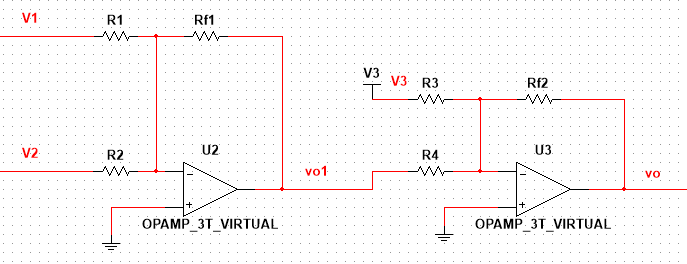
\includegraphics[scale=0.9]{image/C1_a_BT.png}
\end{figure}
a. Ta có:
\[
\left\{
\begin{aligned}
v_{o1} &= -\dfrac{R_{f1}}{R_1}V_1 - \dfrac{R_{f1}}{R_2}V_2 &= -2V_1-3V_2\\
v_o &= -\dfrac{R_{f2}}{R_3}V_3 - \dfrac{R_{f2}}{R4}v_{o1} &= -6V_3-1v_{o1}
\end{aligned}
\right.
\]
Chọn $\boxed{R_{f1}=10K,\; R_{f2}=18K \;\rightarrow\; R_1=5K,\; R_2=3.33K,\; R_3=3K,\; R_4=18K}$
\begin{figure}[H]
	\centering
	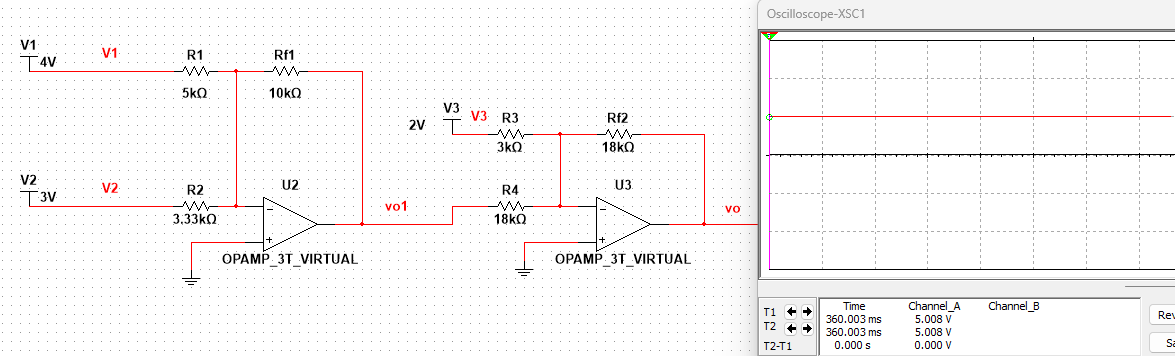
\includegraphics[scale=0.5]{image/C1_simulate.png}
\end{figure}
\textbf{Nhận xét:}\\
- Với $V_1=4V$, $V_2=3V$ ,$V_3=2V$. Theo đề bài, $v_o=5V$ và kết quả mô phỏng được tại $v_o=5.008V$ đúng với yêu cầu thiết kế.\\

b.

\section{Câu 2}


\section{Câu 3}

\section{Câu 4}

\section{Câu 5}

\section{Câu 6}

\section{Câu 7}

\section{Câu 8}
Cho một tín hiệu cần xử lý dưới dạng dòng điện, có tầm thay đổi từ 1mA -- 10mA.

a. Thiết kế mạch cho ngõ ra tầm 0V -- 5V.

b. Lựa chọn OPAMP và các linh kiện cần thiết để mạch hoạt động. Lưu ý: xử lý các
thông số không lý tưởng của OPAMP. (Tham khảo datasheet)

\begin{center}
\textbf{Bài giải}
\end{center}

a. Để thiết kế mạch chuyển đổi tín hiệu dòng điện sang điện áp ta biểu diễn mối quan hệ giữa dòng điện và điện áp như hình bên dưới
\begin{figure}[H]
    \centering
    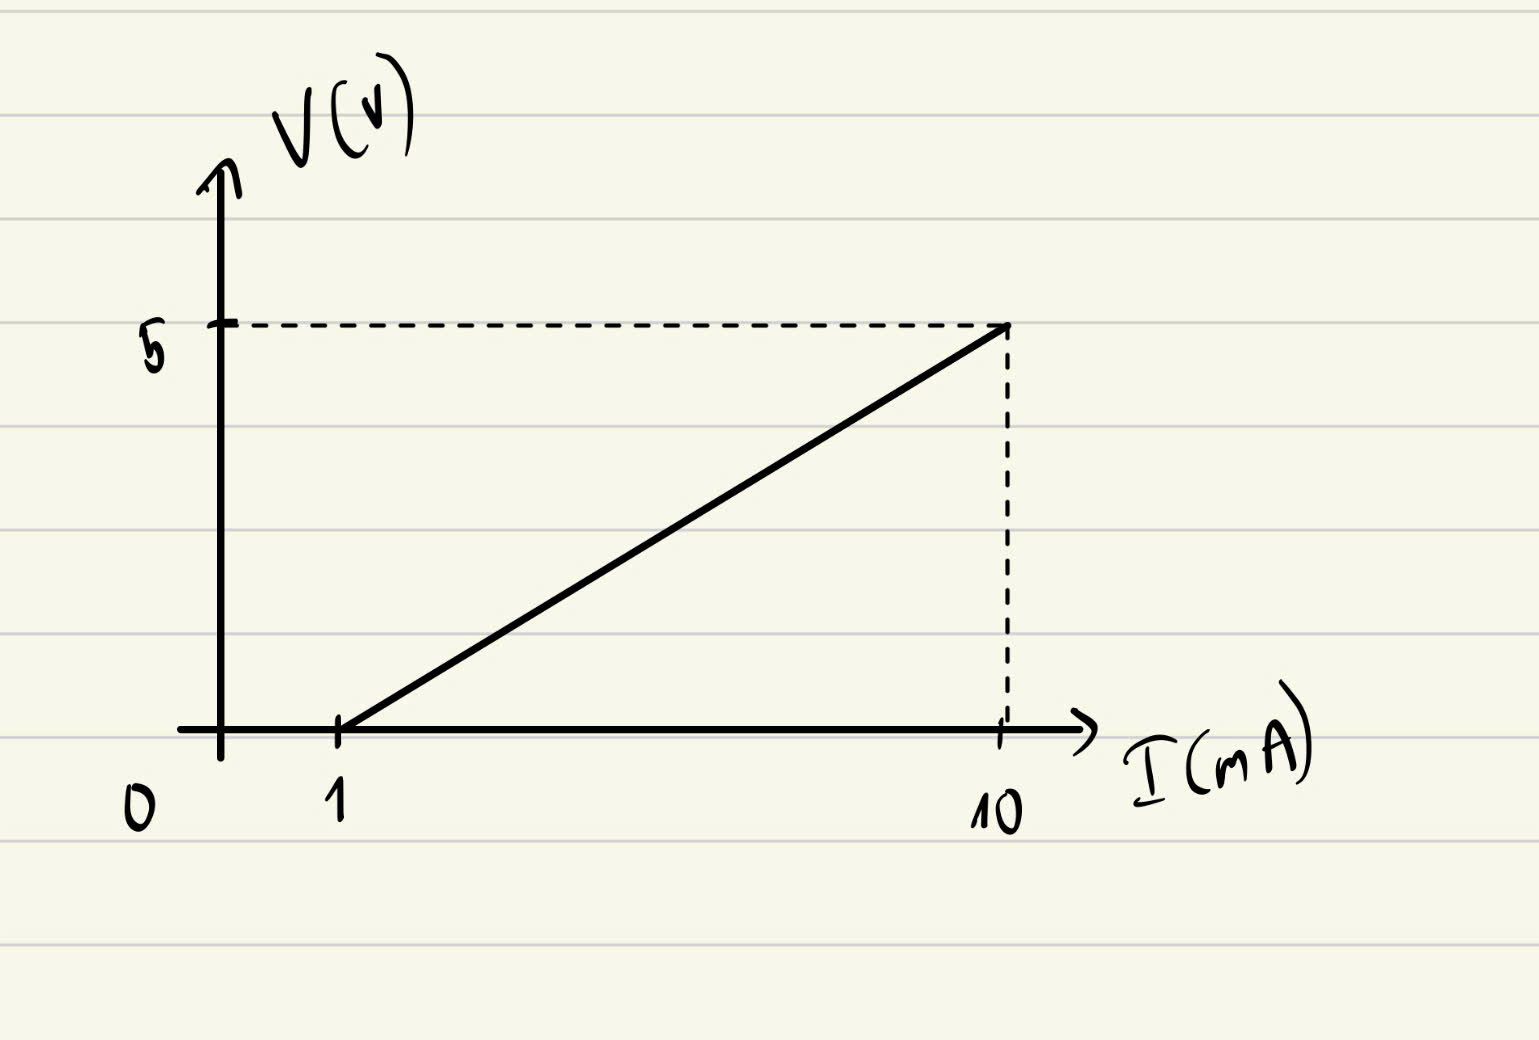
\includegraphics[scale=0.2]{image/C8_chart.png} 
\end{figure}
Từ hình trên ta có hệ phương trình:
\begin{equation*}
    \begin{cases}
        0 = 1\cdot a + b  \\
        5 = 10\cdot a + b\\
    \end{cases}
\end{equation*}
Giải hệ phương trình ta được:  
\begin{equation*}
    \begin{cases}
        a = \dfrac{5}{9} \\
        b = -\dfrac{5}{9} \\
    \end{cases}
\end{equation*}
Vậy ta có phương trình mạch chuyển đổi dòng điện sang điện áp như sau:
\begin{equation*}
    \boxed{V = \dfrac{5}{9}I + \dfrac{5}{9}}
\end{equation*}
\textbf{b.} Thiết kế mạch

Từ phương trình trên
Dùng 1 OPAMP (OPA2333) để làm mạch đảo pha điện áp 5/9 thành điện áp -5/9V.

Dùng 1 OPAMP (LM358P) chuyển đổi dòng thành áp theo tỉ lệ 5/9 V/mA.

Dùng 1 OPAMP (OPA233) cộng 2 điện áp lại với nhau.
Ở mạch U2A, dùng mạch chia áp với nguồn 5.5V để tạo điện áp tham chiếu ngõ vào là $\dfrac{5}{9}V$. Chọn các điện trở:
\begin{equation*}
    R_9 = 760\,\Omega,\quad R_{10} = 100\,\Omega
\end{equation*}


Việc chọn giá trị điện trở được thực hiện như sau:
\begin{itemize}
    \item Các điện trở R$_1$, R$_3$, R$_4$, R$_5$ trong mạch khuếch đại chọn bằng 560\,$\Omega$ để đảm bảo tỉ lệ khuếch đại.
    \item Các điện trở phân cực và hồi tiếp khác chọn giá trị $560\,\Omega$ để giảm thiểu ảnh hưởng của dòng bias.
\end{itemize}
Chọn OPAMP LM358P vì các thông số tham khảo được:
\begin{itemize}
    \item Vsupply : 3V -- 32V, phù hợp với nguồn cấp phổ biến.
    \item Vos (độ dịch chuyển ngõ vào): 2mV.
    \item Ib (dòng dịch chuyển ngõ vào): 2nA.
    \item Ios (dòng dịch chuyển bù ngõ vào): 20nA (max).
\end{itemize}
Chọn OPAMP OPA2333 vì các thông số tham khảo được:
\begin{itemize}
    \item Khả năng rail to rail ở ngõ ra: có.
    \item Vos (độ dịch chuyển ngõ vào): 2$\mu $V.
    \item Ib (dòng dịch chuyển ngõ vào): 2pA.
    \item Ios (dòng dịch chuyển bù ngõ vào): 140pA.
    \item Các sai số ngõ vào rất bé nhưng nguồn cấp khá nhỏ.
\end{itemize}
Mạch hoàn chỉnh như hình bên dưới:
\begin{figure}[H]
    \centering
    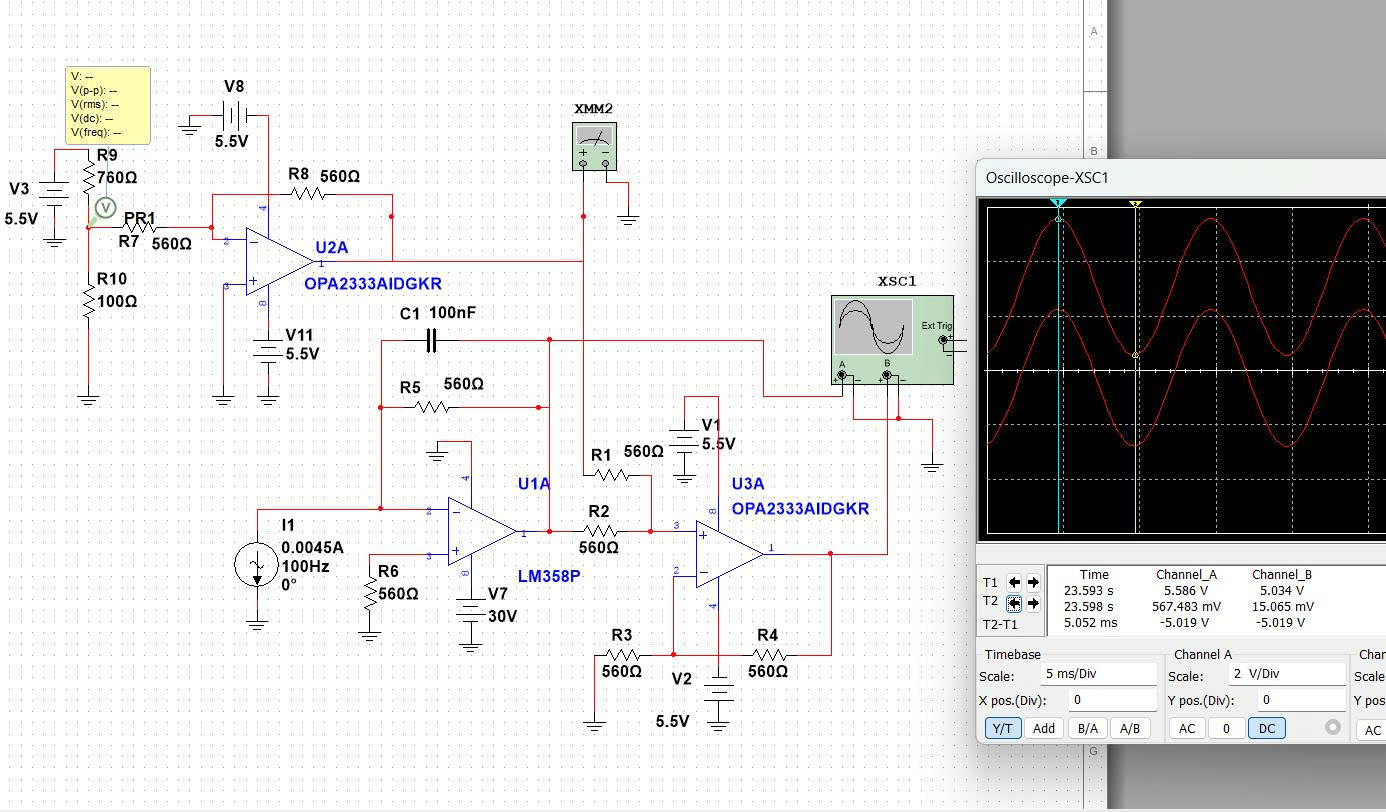
\includegraphics[scale=0.32]{image/C8.png}
\end{figure}
\section{Câu 9}

\section{Câu 10}
Thiết kế mạch dao động tạo sóng vuông đối xứng có chu kỳ 100KHz, chỉ dùng 1
OPAMP, các điện trở và tụ.

\begin{center}
\textbf{Bài giải}
\end{center}

Áp dụng kiến thức tạo xung bằng OPAMP sử dụng mạch với cả 2 hồi tiếp âm và dương như hình bên dưới.
\begin{figure}[H]
    \centering
    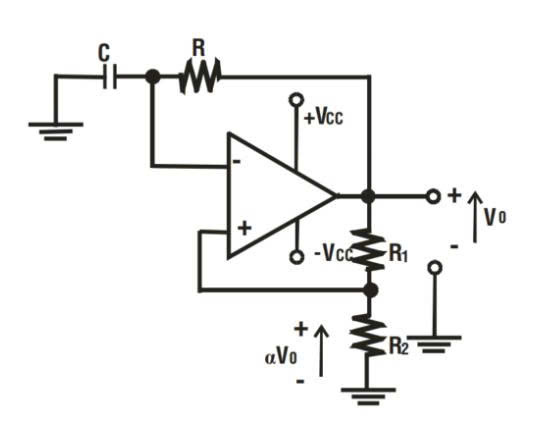
\includegraphics[scale=0.6]{image/StandardDesign_Cau10.png}
\end{figure}
Điều kiện đề bài cho là phải thiết kế mạch tạo sóng vuông đối xứng 100KHz nên ta có:
\begin{equation*}
    T = \dfrac{1}{f} = 10\mu s
\end{equation*}
\begin{equation*}
    T = T_1 + T_2 = 2T_1 = 2RC\ln\dfrac{1+\alpha}{1-\alpha}
\end{equation*}
\begin{equation*}
    \text{Với }  \alpha = \dfrac{R_2}{R_1 + R_2}
\end{equation*}
Từ dạng OPAMP trên ta chọn các thông số:
\begin{equation*}
    R_2 = 1k\Omega
\end{equation*}
\begin{equation*}
    R_3 = 1k\Omega
\end{equation*}
\begin{equation*}
    \alpha = \dfrac{1}{2}
\end{equation*}
\begin{equation*}
    \rightarrow T_1 = RC\ln 3
\end{equation*}
\begin{equation*}
    \rightarrow 10\mu s = 2RC\ln 3
\end{equation*}
\begin{equation*}
    \rightarrow RC = \dfrac{10\mu s}{2\ln 3} = 4.55\mu s
\end{equation*}
\begin{equation*}
    \text{Chọn } R_1 = 1k\Omega
\end{equation*}
\begin{equation*}
    \rightarrow C = 4.5nF
\end{equation*}

Chọn OPAMP LM7171AIM vì các thông số tham khảo được: \\
- Băng thông: 200MHz\\
- Slew Rate: 4100V/$\mu s$, phù hợp cho mạch so sánh và chuyển mạch nhanh\\
- Độ trễ ngõ ra so với ngõ vào thấp, phù hợp cho mạch tạo xung ổn định.\\
Mô phỏng mạch thu được kết quả:
\begin{figure}[H]
    \centering
    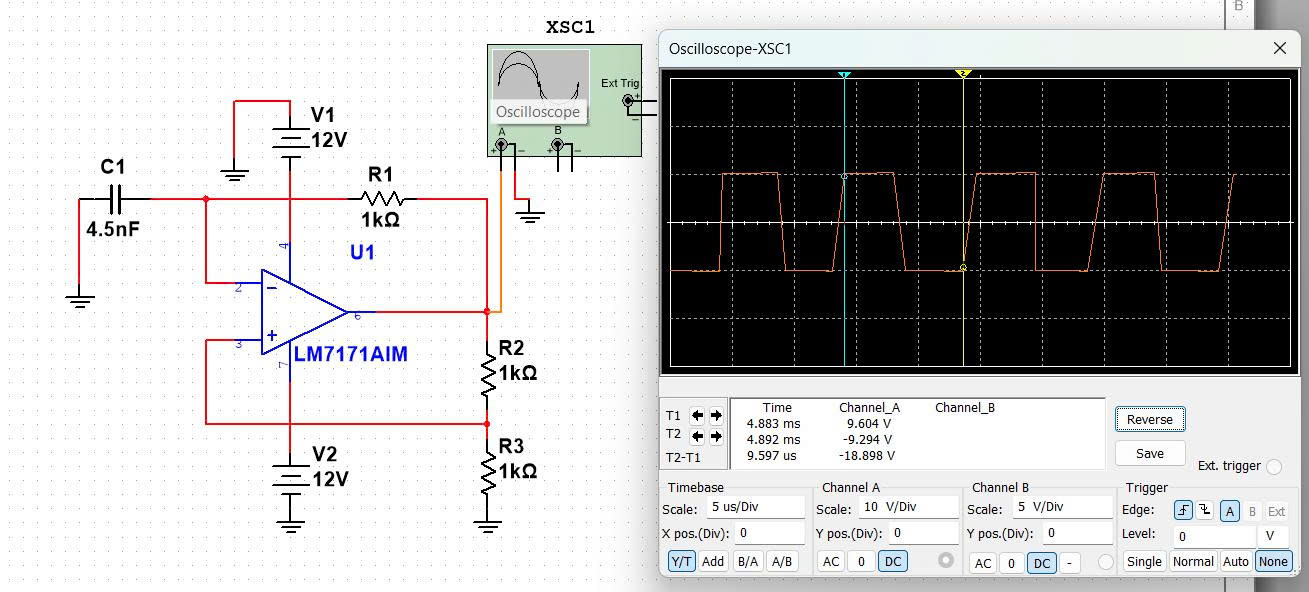
\includegraphics[scale=0.3]{image/C10.png}
\end{figure}
\section{Câu 11}
Thiết kế mạch Schmitt Trigger thực hiện đặc tuyến như ở hình 6a và 6b. (Mỗi hình 1
mạch, coi OPAMP là lý tưởng)
\begin{figure}[H]
	\centering
	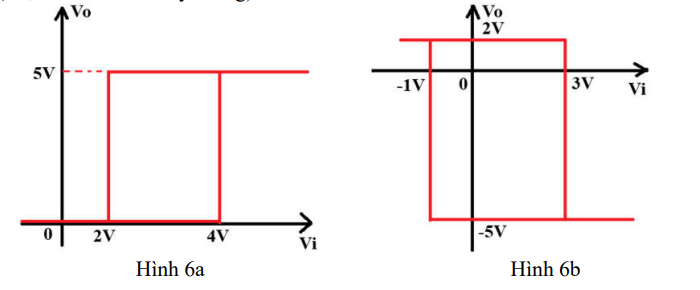
\includegraphics[scale=0.6]{image/C11_De.png}
\end{figure}

\begin{center}
\textbf{Bài giải}
\end{center}

\textbf{Hình 6a}\\
Dùng mạch Schmitt Trigger không đảo
\begin{figure}[H]
	\centering
	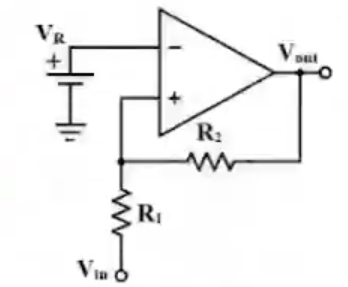
\includegraphics[scale=0.55]{image/C11_Trigger_Ko_Dao.png}
\end{figure}
Ta có:
\begin{align*}
	V_{DB} &= V_{UT} - V_{LT} = (V_{OH}-V_{OL})\dfrac{R_1}{R_2}
	&\hspace{0cm}\text{Với}\quad
	\left\{
	\begin{aligned}
		V_{UT} &= 4V\\
		V_{LT} &= 2V\\
		V_{OH} &= 5V\\
		V_{OL} &= 0V
	\end{aligned}
	\right.\\
	\rightarrow\quad   2 &= 5 \cdot \dfrac{R_1}{R_2} \quad
    \rightarrow\quad \dfrac{R_1}{R_2} = \dfrac{2}{5} 
\end{align*}

Chọn
\boxed{%
\left\{
\begin{aligned}
R_1 &= 2\ \mathrm{k}\Omega\\
R_2 &= 5\ \mathrm{k}\Omega
\end{aligned}
\right.
}\\

Có: $V_{LT} = V_R\left(1+\dfrac{R_1}{R_2}\right) - V_{OH}\dfrac{R_1}{R_2} \quad \rightarrow \quad \boxed{V_R = 2.857V}$

Mô phỏng:
\begin{figure}[H]
	\centering
	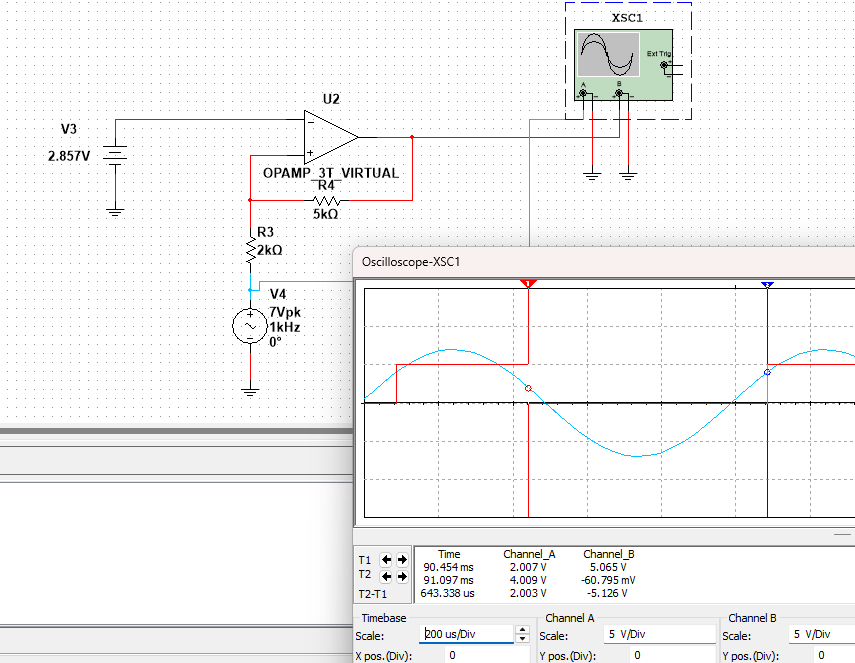
\includegraphics[scale=0.5]{image/C11_6a.png}
\end{figure}
\textbf{Nhận xét:} Với signal màu xanh là input và đỏ là ouput, có thể thấy $V_{UT}=4.009V, V_{LT}=2.007V, V_{OH}=5.065V, V_{OL}=-0.068V$ đã đúng với yêu cầu thiết kế.
Khi $V_i>V_{UT}$ thì $V_o=V_{OH}$ và khi $V_i<V_{LT}$ thì $V_o=V_{OL}$.\\

\textbf{Hình 6b}\\
Dùng mạch Schmitt Trigger đảo
\begin{figure}[H]
	\centering
	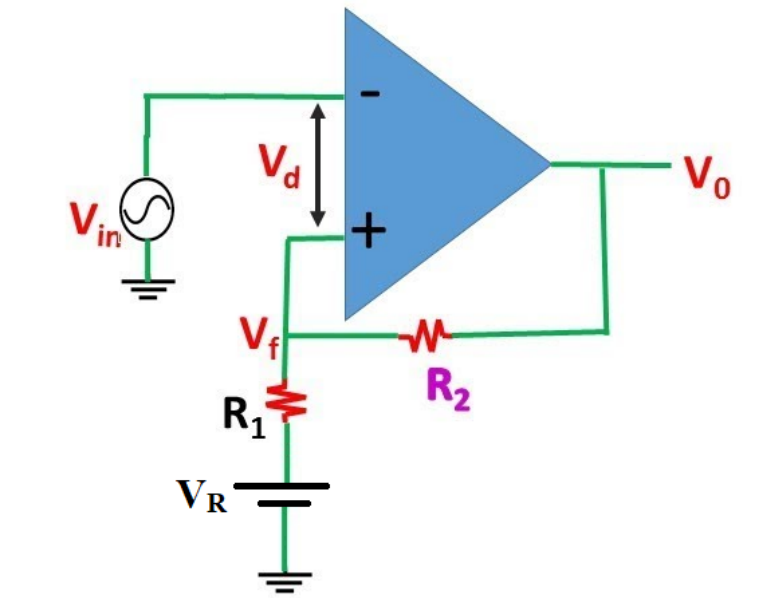
\includegraphics[scale=0.5]{image/C11_Trigger_Dao.png}
\end{figure}
Ta có:
\begin{align*}
	V_{DB} &= V_{UT} - V_{LT} = (V_{OH}-V_{OL})\dfrac{R_1}{R_1+R_2}
	&\hspace{0cm}\text{Với}\quad
	\left\{
	\begin{aligned}
		V_{UT} &= 3V\\
		V_{LT} &= -1V\\
		V_{OH} &= 2V\\
		V_{OL} &= -5V
	\end{aligned}
	\right.\\
	\rightarrow\quad   4 &= 7 \cdot \dfrac{R_1}{R_1+R_2} \quad
    \rightarrow\quad R_1 = \dfrac{4}{3}R_2  
\end{align*}

Chọn
\boxed{%
\left\{
\begin{aligned}
R_1 &= 4\ \mathrm{k}\Omega\\
R_2 &= 3\ \mathrm{k}\Omega
\end{aligned}
\right.
}\\

Có: $V_{LT} = \dfrac{V_{OL}R_1 + V_RR_2}{R_1+R_2} \quad \rightarrow \quad \boxed{V_R = 4.333V}$\\

Mô phỏng:
\begin{figure}[H]
	\centering
	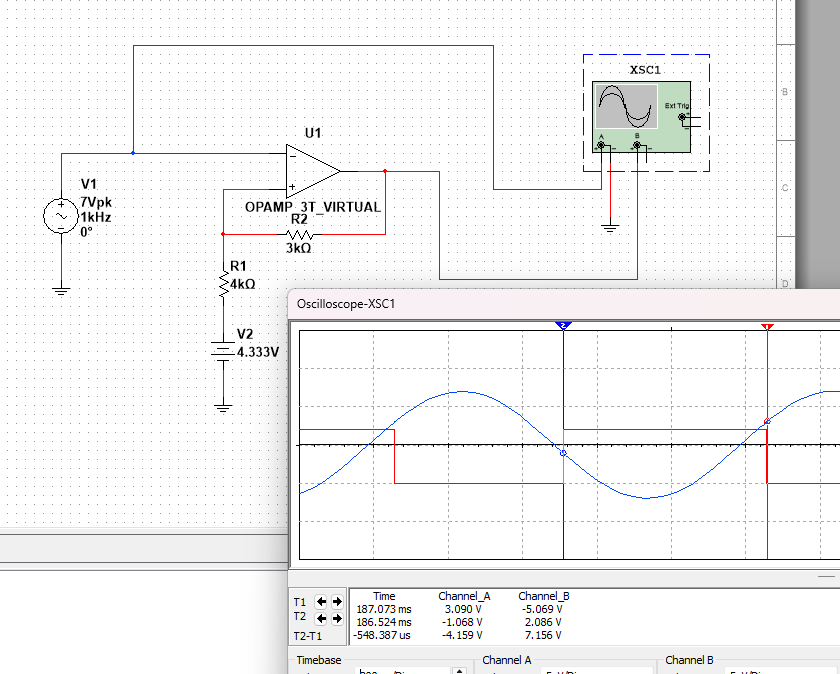
\includegraphics[scale=0.5]{image/C11_6b.png}
\end{figure}
\textbf{Nhận xét:} Với signal màu xanh là input và đỏ là ouput, có thể thấy $V_{UT}=3.090V, V_{LT}=-1.068V, V_{OH}=2.086V, V_{OL}=-5.069V$ đã đúng với yêu cầu thiết kế.
Khi $V_i>V_{UT}$ thì $V_o=V_{OL}$ và khi $V_i<V_{LT}$ thì $V_o=V_{OH}$.

\section{Câu 12}

\section{Câu 13}
Cho mạch điện như ở Hình 8a. OPAMP được cấp nguồn có $V_{OH}=3.3V$, $V_{OL}=-3V$.
Các điện trở được chọn $R_1=2K$, $R_2=3K$, $R_3=4K$, $R_4=6K$.\\
Cho dạng sóng Vi(t) như ở Hình 8b. Vẽ dạng sóng ngõ ra Vo trong các trường hợp sau:\\
a. $V_1=2V$, $V_{m1}=2V$, $V_{m2}=-3V$\\
b. $V_1=4V$, $V_{m1}=1V$, $V_{m2}=-3V$
\begin{figure}[H]
	\centering
	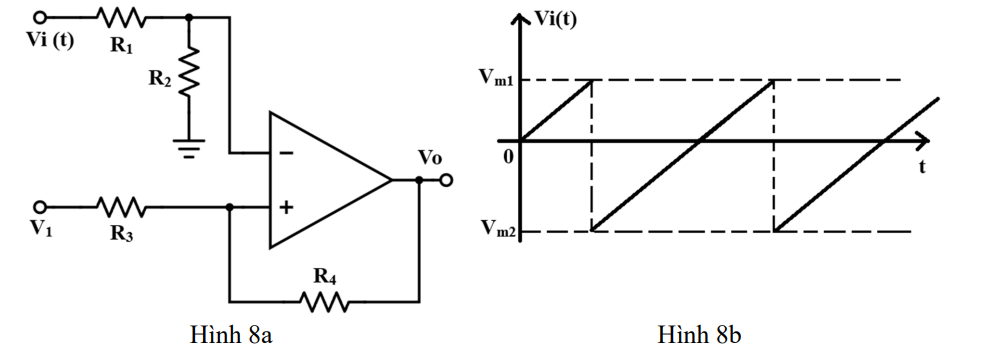
\includegraphics[scale=0.9]{image/C13_De.png}
\end{figure}
\begin{center}
\textbf{Bài giải}
\end{center}
a. Giả sử OPAMP lý tưởng:\\
Ta có:
\[
\left\{
\begin{aligned}
V^- &= \dfrac{R_2}{R_1+R_2}V_i \\
V^+ &= \dfrac{\dfrac{V_1}{R_3} + \dfrac{V_o}{R_2}}{\dfrac{1}{R_3} + \dfrac{1}{R_4}} = \dfrac{3}{5}V_1 +\dfrac{2}{5}V_o
\end{aligned}
\right.
\]

\[
\begin{aligned}
&\text{Giả sử }& V_o = V_{OH} &\qquad\rightarrow\qquad V^+ = \dfrac{3}{5}\cdot2 + \dfrac{2}{5}\cdot3.3 \quad;\quad V^- = 0.6V_i \\
&\text{Để }& V_o = V_{OL} &\qquad\rightarrow\qquad V^+ < V^- \quad\rightarrow\quad \boxed{V_i>4.2V}\\
&\rightarrow& V_o = V_{OL} &\qquad\rightarrow\qquad V^+ = \dfrac{3}{5}\cdot2 + \dfrac{2}{5}\cdot-3 \quad;\quad V^- = 0.6V_i \\
&\text{Để }& V_o = V_{OH} &\qquad\rightarrow\qquad V^+ > V^- \quad\rightarrow\quad \boxed{V_i<0V}\\
\end{aligned}
\]\\
Tại t=0 đến khi $V_i(t)=0$ nằm trong khoảng Deadband của OPAMP. Vì thế tùy vào trạng thái ban đầu sẽ cho ra ngõ ra khác nhau.
Sau khi $V_i(t)<0$ thì $V_o = V_{OH}$ và $V_i$ luôn bé hơn 4.2V nên không thể cho $V_o=V_{OL}$. Vì thế nên $V_o$ từ đó luôn bằng $V_{OH}$
\begin{figure}[H]
	\centering
	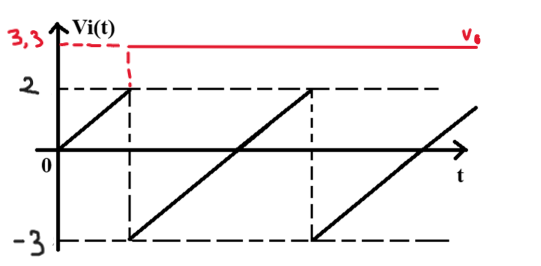
\includegraphics[scale=1]{image/C13_a_BT.png}
\end{figure}

\begin{figure}[H]
    \centering
    \begin{subfigure}[b]{0.48\textwidth}
        \centering
        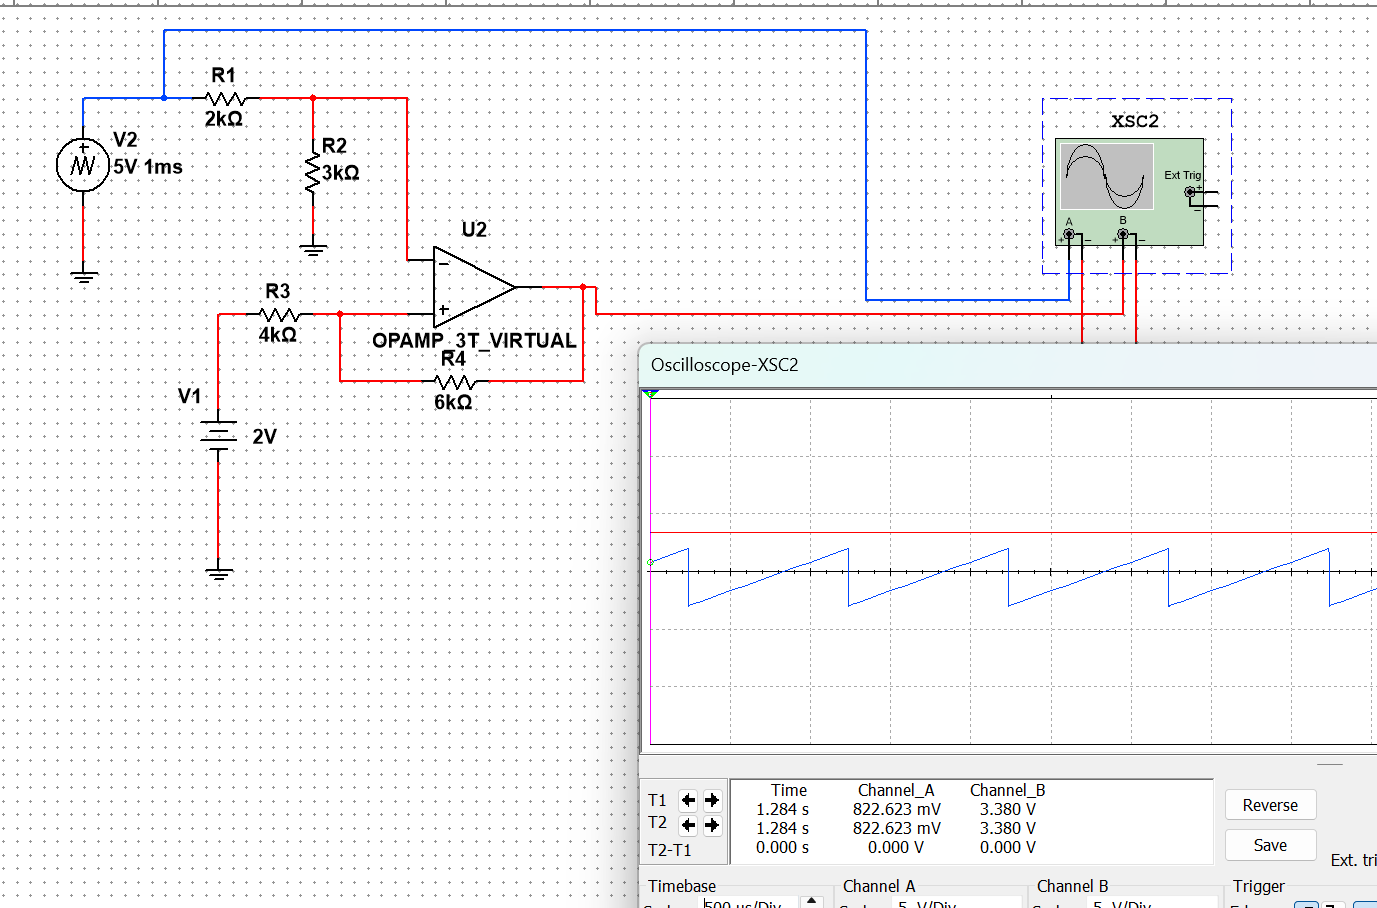
\includegraphics[width=\textwidth]{image/C13_a.png}
        \caption*{Hình a1}
    \end{subfigure}
    \hfill
    \begin{subfigure}[b]{0.48\textwidth}
        \centering
        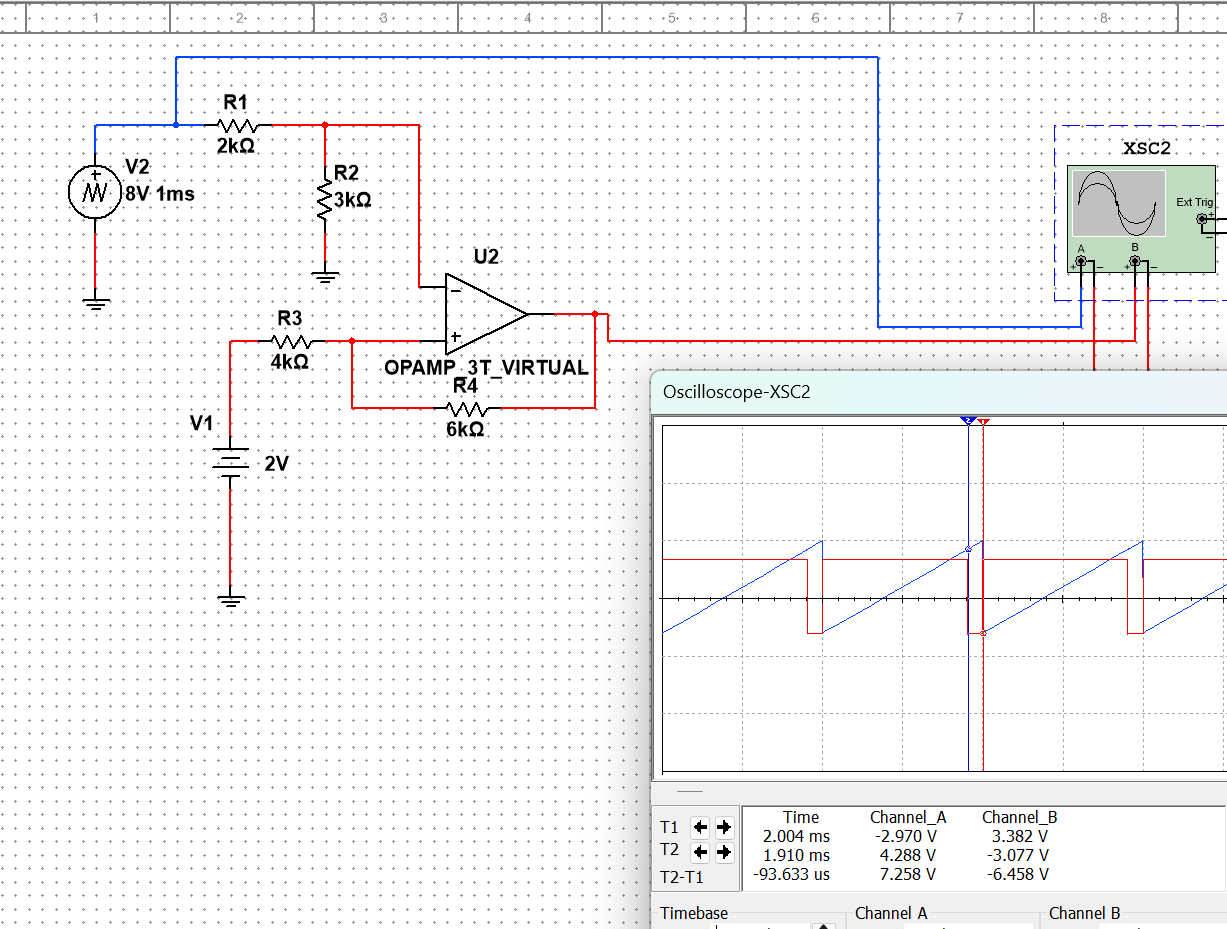
\includegraphics[width=\textwidth]{image/C13_a_1.png}
        \caption*{Hình a2}
    \end{subfigure}
\end{figure}

\textbf{Nhận xét:}\\
- Hình a1 mô phỏng $V_i$ theo đề bài với màu xanh, $V_o=-3.380V$ màu đỏ xấp xỉ 3.3V đúng với tính toán.\\
- Hình a2 chọn $V_i(t)$ thỏa $V_i>V_{UT}$ và $V_i<V_{LT}$ để kiểm tra lại $V_{UT}=4.288V$ và $V_{LT}=-2.970V$. 
Theo kết quả mô phỏng được có thể thấy $V_{UT}$ xấp xỉ 4.2V, còn $V_{LT}$ do độ dốc lớn nên không thể đo chính xác được.\\

b. Giả sử OPAMP lý tưởng:\\
Ta có:
\[
\left\{
\begin{aligned}
V^- &= \dfrac{R_2}{R_1+R_2}V_i \\
V^+ &= \dfrac{\dfrac{V_1}{R_3} + \dfrac{V_o}{R_2}}{\dfrac{1}{R_3} + \dfrac{1}{R_4}} = \dfrac{3}{5}V_1 +\dfrac{2}{5}V_o
\end{aligned}
\right.
\]

\[
\begin{aligned}
&\text{Giả sử }& V_o = V_{OH} &\qquad\rightarrow\qquad V^+ = \dfrac{3}{5}\cdot4 + \dfrac{2}{5}\cdot3.3 \quad;\quad V^- = 0.6V_i \\
&\text{Để }& V_o = V_{OL} &\qquad\rightarrow\qquad V^+ < V^- \quad\rightarrow\quad \boxed{V_i>6.2V}\\
&\rightarrow& V_o = V_{OL} &\qquad\rightarrow\qquad V^+ = \dfrac{3}{5}\cdot4 + \dfrac{2}{5}\cdot-3 \quad;\quad V^- = 0.6V_i \\
&\text{Để }& V_o = V_{OH} &\qquad\rightarrow\qquad V^+ > V^- \quad\rightarrow\quad \boxed{V_i<2V}\\
\end{aligned}
\]\\
Tại t=0 đến khi $V_i(t)=0$ nằm trong khoảng Deadband của OPAMP. Vì thế tùy vào trạng thái ban đầu sẽ cho ra ngõ ra khác nhau.
Sau khi $V_i(t)<0$ thì $V_o = V_{OH}$ và $V_i$ luôn bé hơn 6.2V nên không thể cho $V_o=V_{OL}$. Vì thế nên $V_o$ từ đó luôn bằng $V_{OH}$
\begin{figure}[H]
	\centering
	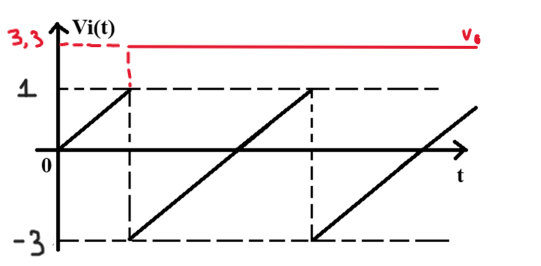
\includegraphics[scale=1]{image/C13_b_BT.png}
\end{figure}

\begin{figure}[H]
    \centering
    \begin{subfigure}[b]{0.48\textwidth}
        \centering
        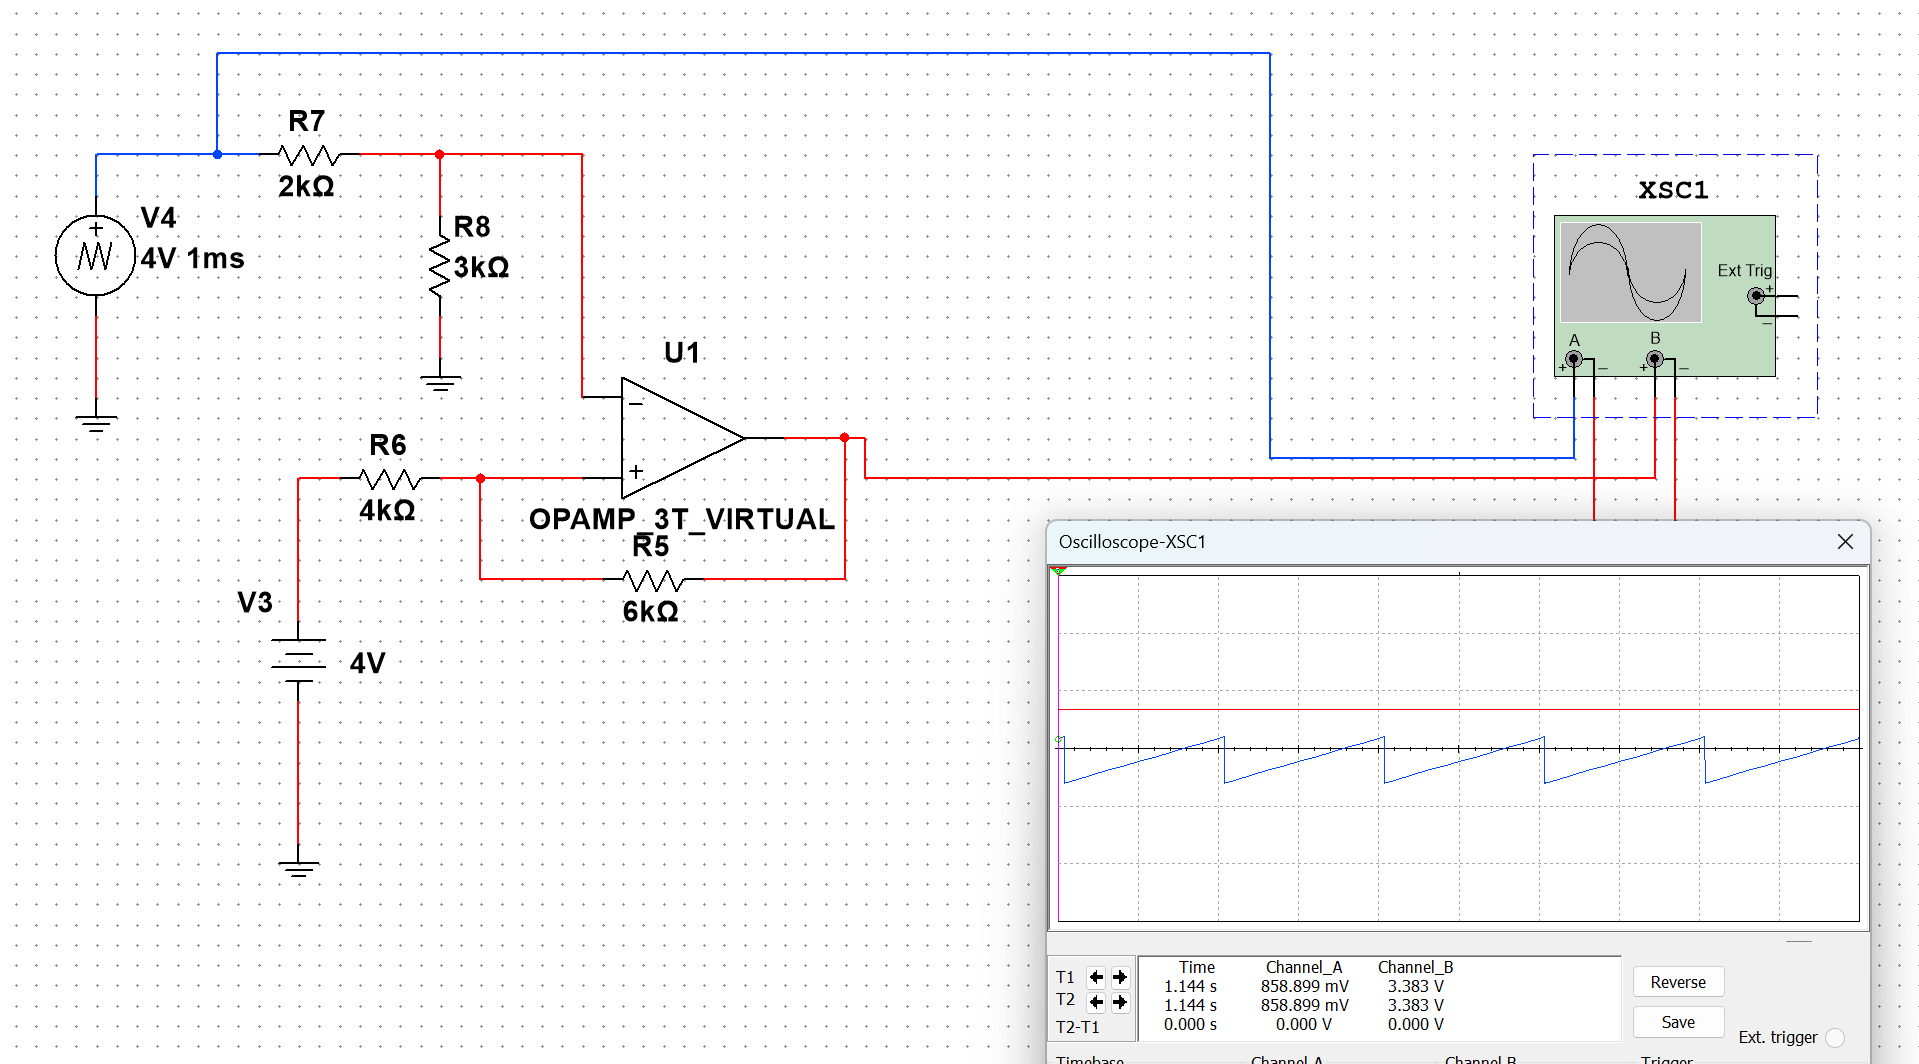
\includegraphics[width=\textwidth]{image/C13_b.png}
        \caption*{Hình b1}
    \end{subfigure}
    \hfill
    \begin{subfigure}[b]{0.48\textwidth}
        \centering
        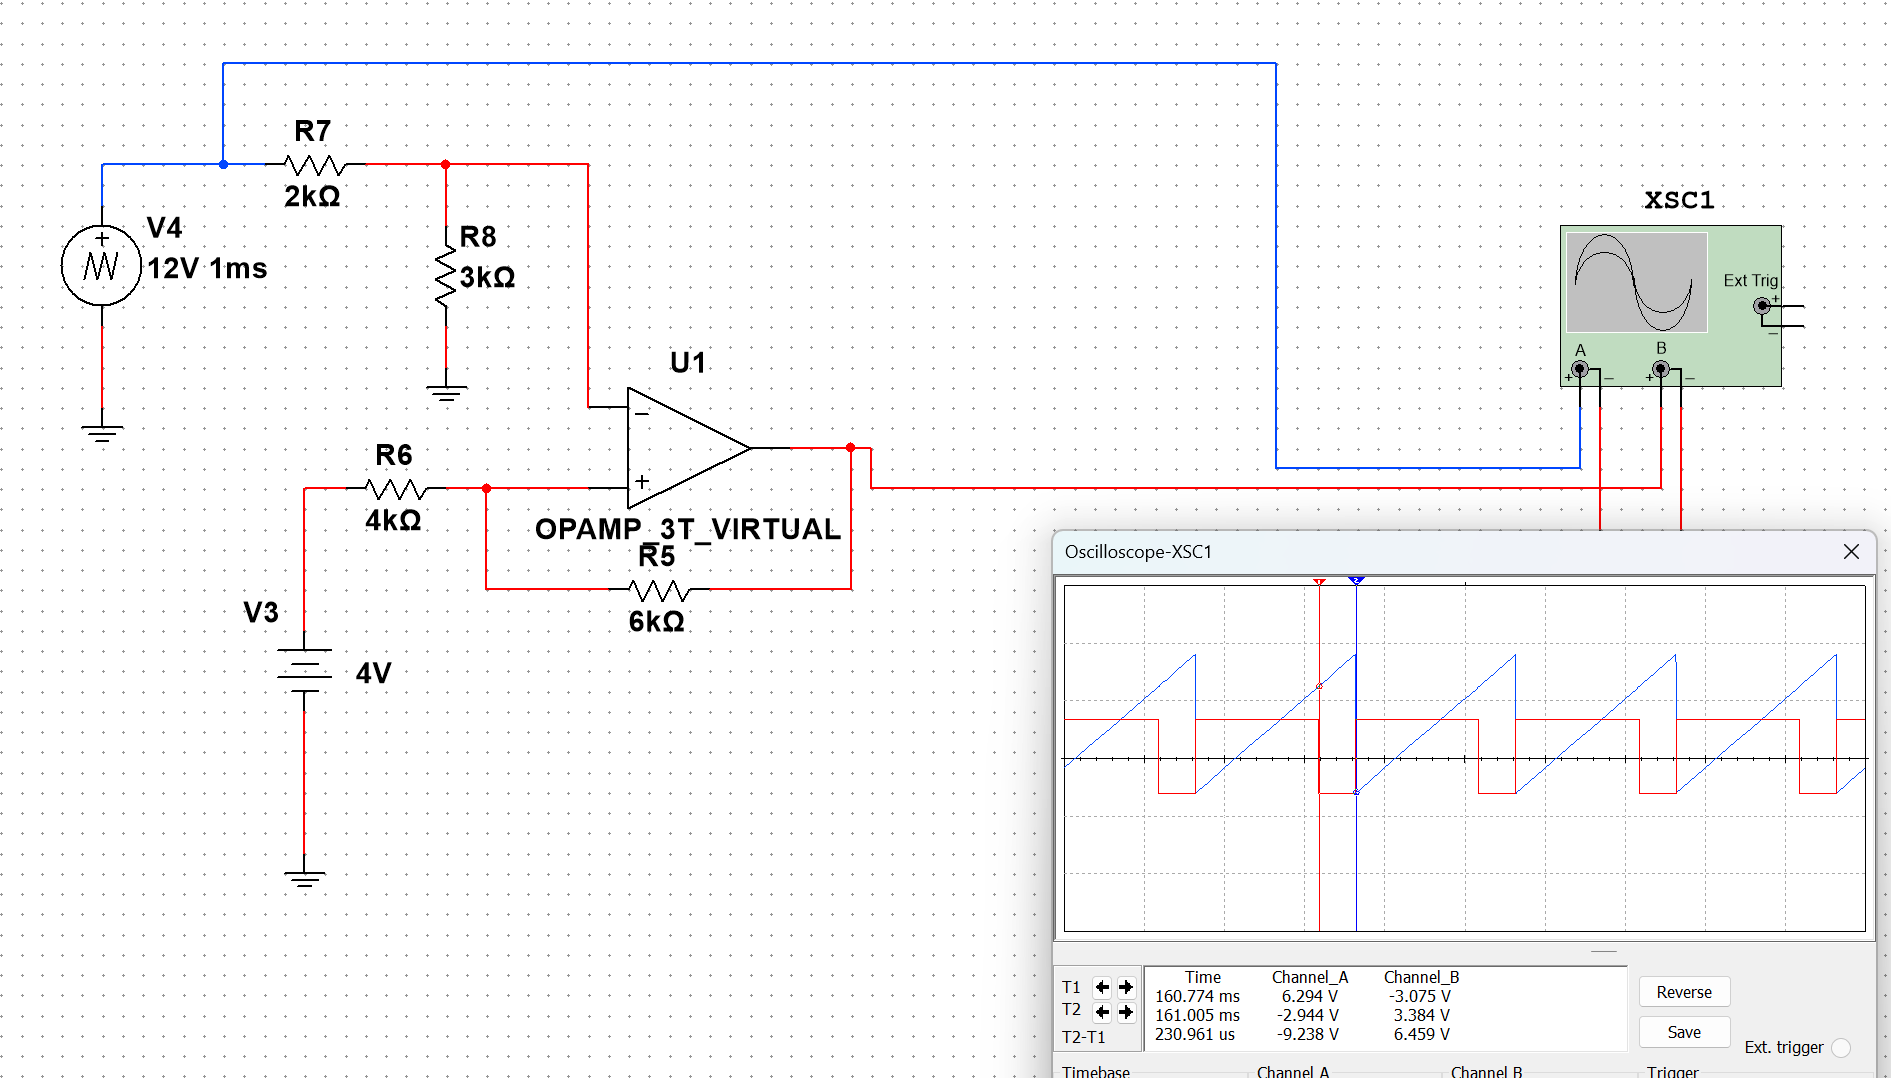
\includegraphics[width=\textwidth]{image/C13_b_1.png}
        \caption*{Hình b2}
    \end{subfigure}
\end{figure}

\textbf{Nhận xét:}\\
- Hình a1 mô phỏng $V_i$ theo đề bài với màu xanh, $V_o=-3.383V$ màu đỏ xấp xỉ 3.3V đúng với tính toán.\\
- Hình a2 chọn $V_i(t)$ thỏa $V_i>V_{UT}$ và $V_i<V_{LT}$ để kiểm tra lại $V_{UT}=6.294V$ và $V_{LT}=-2.944V$. 
Theo kết quả mô phỏng được có thể thấy $V_{UT}$ xấp xỉ 6.2V, còn $V_{LT}$ do độ dốc lớn nên không thể đo chính xác được.\\

\section{Câu 14}



\end{document}